% Options for packages loaded elsewhere
\PassOptionsToPackage{unicode}{hyperref}
\PassOptionsToPackage{hyphens}{url}
%
\documentclass[
]{article}
\usepackage{amsmath,amssymb}
\usepackage{lmodern}
\usepackage{iftex}
\ifPDFTeX
  \usepackage[T1]{fontenc}
  \usepackage[utf8]{inputenc}
  \usepackage{textcomp} % provide euro and other symbols
\else % if luatex or xetex
  \usepackage{unicode-math}
  \defaultfontfeatures{Scale=MatchLowercase}
  \defaultfontfeatures[\rmfamily]{Ligatures=TeX,Scale=1}
\fi
% Use upquote if available, for straight quotes in verbatim environments
\IfFileExists{upquote.sty}{\usepackage{upquote}}{}
\IfFileExists{microtype.sty}{% use microtype if available
  \usepackage[]{microtype}
  \UseMicrotypeSet[protrusion]{basicmath} % disable protrusion for tt fonts
}{}
\makeatletter
\@ifundefined{KOMAClassName}{% if non-KOMA class
  \IfFileExists{parskip.sty}{%
    \usepackage{parskip}
  }{% else
    \setlength{\parindent}{0pt}
    \setlength{\parskip}{6pt plus 2pt minus 1pt}}
}{% if KOMA class
  \KOMAoptions{parskip=half}}
\makeatother
\usepackage{xcolor}
\usepackage[margin=1in]{geometry}
\usepackage{color}
\usepackage{fancyvrb}
\newcommand{\VerbBar}{|}
\newcommand{\VERB}{\Verb[commandchars=\\\{\}]}
\DefineVerbatimEnvironment{Highlighting}{Verbatim}{commandchars=\\\{\}}
% Add ',fontsize=\small' for more characters per line
\usepackage{framed}
\definecolor{shadecolor}{RGB}{248,248,248}
\newenvironment{Shaded}{\begin{snugshade}}{\end{snugshade}}
\newcommand{\AlertTok}[1]{\textcolor[rgb]{0.94,0.16,0.16}{#1}}
\newcommand{\AnnotationTok}[1]{\textcolor[rgb]{0.56,0.35,0.01}{\textbf{\textit{#1}}}}
\newcommand{\AttributeTok}[1]{\textcolor[rgb]{0.77,0.63,0.00}{#1}}
\newcommand{\BaseNTok}[1]{\textcolor[rgb]{0.00,0.00,0.81}{#1}}
\newcommand{\BuiltInTok}[1]{#1}
\newcommand{\CharTok}[1]{\textcolor[rgb]{0.31,0.60,0.02}{#1}}
\newcommand{\CommentTok}[1]{\textcolor[rgb]{0.56,0.35,0.01}{\textit{#1}}}
\newcommand{\CommentVarTok}[1]{\textcolor[rgb]{0.56,0.35,0.01}{\textbf{\textit{#1}}}}
\newcommand{\ConstantTok}[1]{\textcolor[rgb]{0.00,0.00,0.00}{#1}}
\newcommand{\ControlFlowTok}[1]{\textcolor[rgb]{0.13,0.29,0.53}{\textbf{#1}}}
\newcommand{\DataTypeTok}[1]{\textcolor[rgb]{0.13,0.29,0.53}{#1}}
\newcommand{\DecValTok}[1]{\textcolor[rgb]{0.00,0.00,0.81}{#1}}
\newcommand{\DocumentationTok}[1]{\textcolor[rgb]{0.56,0.35,0.01}{\textbf{\textit{#1}}}}
\newcommand{\ErrorTok}[1]{\textcolor[rgb]{0.64,0.00,0.00}{\textbf{#1}}}
\newcommand{\ExtensionTok}[1]{#1}
\newcommand{\FloatTok}[1]{\textcolor[rgb]{0.00,0.00,0.81}{#1}}
\newcommand{\FunctionTok}[1]{\textcolor[rgb]{0.00,0.00,0.00}{#1}}
\newcommand{\ImportTok}[1]{#1}
\newcommand{\InformationTok}[1]{\textcolor[rgb]{0.56,0.35,0.01}{\textbf{\textit{#1}}}}
\newcommand{\KeywordTok}[1]{\textcolor[rgb]{0.13,0.29,0.53}{\textbf{#1}}}
\newcommand{\NormalTok}[1]{#1}
\newcommand{\OperatorTok}[1]{\textcolor[rgb]{0.81,0.36,0.00}{\textbf{#1}}}
\newcommand{\OtherTok}[1]{\textcolor[rgb]{0.56,0.35,0.01}{#1}}
\newcommand{\PreprocessorTok}[1]{\textcolor[rgb]{0.56,0.35,0.01}{\textit{#1}}}
\newcommand{\RegionMarkerTok}[1]{#1}
\newcommand{\SpecialCharTok}[1]{\textcolor[rgb]{0.00,0.00,0.00}{#1}}
\newcommand{\SpecialStringTok}[1]{\textcolor[rgb]{0.31,0.60,0.02}{#1}}
\newcommand{\StringTok}[1]{\textcolor[rgb]{0.31,0.60,0.02}{#1}}
\newcommand{\VariableTok}[1]{\textcolor[rgb]{0.00,0.00,0.00}{#1}}
\newcommand{\VerbatimStringTok}[1]{\textcolor[rgb]{0.31,0.60,0.02}{#1}}
\newcommand{\WarningTok}[1]{\textcolor[rgb]{0.56,0.35,0.01}{\textbf{\textit{#1}}}}
\usepackage{graphicx}
\makeatletter
\def\maxwidth{\ifdim\Gin@nat@width>\linewidth\linewidth\else\Gin@nat@width\fi}
\def\maxheight{\ifdim\Gin@nat@height>\textheight\textheight\else\Gin@nat@height\fi}
\makeatother
% Scale images if necessary, so that they will not overflow the page
% margins by default, and it is still possible to overwrite the defaults
% using explicit options in \includegraphics[width, height, ...]{}
\setkeys{Gin}{width=\maxwidth,height=\maxheight,keepaspectratio}
% Set default figure placement to htbp
\makeatletter
\def\fps@figure{htbp}
\makeatother
\setlength{\emergencystretch}{3em} % prevent overfull lines
\providecommand{\tightlist}{%
  \setlength{\itemsep}{0pt}\setlength{\parskip}{0pt}}
\setcounter{secnumdepth}{-\maxdimen} % remove section numbering
\ifLuaTeX
  \usepackage{selnolig}  % disable illegal ligatures
\fi
\IfFileExists{bookmark.sty}{\usepackage{bookmark}}{\usepackage{hyperref}}
\IfFileExists{xurl.sty}{\usepackage{xurl}}{} % add URL line breaks if available
\urlstyle{same} % disable monospaced font for URLs
\hypersetup{
  pdftitle={Data Transformation - Out of Class with reading},
  hidelinks,
  pdfcreator={LaTeX via pandoc}}

\title{Data Transformation - Out of Class with reading}
\author{}
\date{\vspace{-2.5em}}

\begin{document}
\maketitle

\hypertarget{connection-to-previous-work-on-data-organization}{%
\subsection{Connection to previous work on Data
Organization}\label{connection-to-previous-work-on-data-organization}}

We will finally see why organized data is worth the effort. We'll follow
an exercise using a data source with over 300,000 rows! The work this
week will show us (1) why R is awesome and fast for analysis, (2)
reinforce the purpose of organized data (following the 12 best practices
we learned in Week 1).

\hypertarget{source}{%
\subsection{Source}\label{source}}

This exercise follows along with the reading for this week R for Data
Science Chapter 5 \url{https://r4ds.had.co.nz/transform.html}. The
template below is for you to be able to follow along in the reading and
complete the exercises.

\hypertarget{section}{%
\subsection{5.1.1}\label{section}}

I've gone ahead and loaded the 2 packages, but you need to turn them
``on''. Below, follow the instructions using :

\begin{Shaded}
\begin{Highlighting}[]
\FunctionTok{library}\NormalTok{(nycflights13)}
\FunctionTok{library}\NormalTok{(tidyverse)}
\end{Highlighting}
\end{Shaded}

\begin{verbatim}
## -- Attaching packages --------------------------------------- tidyverse 1.3.2 --
## v ggplot2 3.4.0     v purrr   1.0.1
## v tibble  3.1.8     v dplyr   1.1.0
## v tidyr   1.3.0     v stringr 1.5.0
## v readr   2.1.3     v forcats 1.0.0
## -- Conflicts ------------------------------------------ tidyverse_conflicts() --
## x dplyr::filter() masks stats::filter()
## x dplyr::lag()    masks stats::lag()
\end{verbatim}

Why is it important to do this? When you are creating code, explicitly
turning on packages that are required is considered good practice. This
goes along with the importance of being intentional and making your code
reproducible by anyone, anywhere. Tell the computer what to
do\ldots explicitly! Tell everyone explicitly when you have done to get
to your results.

This also keeps your R sessions memory low and prevents duplicate
functions from being loaded from different packages. Notice above when
we load tidyverse we get the message that
\texttt{✖\ dplyr::filter()\ masks\ stats::filter()} and
\texttt{✖\ dplyr::lag()\ \ \ \ masks\ stats::lag()}, that is because the
stats package also has filter and lag functions as well as the dplyr
package which is part of the tidyverse package. The tidyverse is
actually a package of packages including ggplot2, purrr, tibble, dplyr,
tidyr, stringr, readr, and forcats. We will learn more about all of
these in coming weeks. In our case, because we more recently loaded
tidyverse if we call \texttt{filter(some\_argument...)} this will run
the tidyverse/dplyr version of the function. As it says in
\href{https://r4ds.had.co.nz/transform.html\#prerequisites-2}{the
reading}, if you want to use the base, or stats, version of these
functions after loading dplyr, you'll need to specify the package that
the function comes from using two colons \texttt{::} as in
\texttt{stats::filter()} and \texttt{stats::lag().}

\hypertarget{section-1}{%
\subsection{5.1.2}\label{section-1}}

Run \texttt{flights} in the code chunk below. The output should match
the reading. Note that you can find a nice README/data
dictionary/documentation of this dataset by viewing its help
documentation \texttt{?flights}.

As described, \texttt{flights} is a data frame called a tibble. What
does \texttt{int} mean on the third line of the table? Or \texttt{dbl}?

These are types of variables. Be sure to familiarize yourself with the
various types as you move forward, so focus on this section in
\href{https://r4ds.had.co.nz/transform.html\#prerequisites-2}{the
reading}. You can also check out
\href{https://datacarpentry.org/R-ecology-lesson/01-intro-to-r.html\#Vectors_and_data_types}{Vectors
and data types in Data Carpentry}.

\hypertarget{dplyr-basics}{%
\subsection{dplyr basics}\label{dplyr-basics}}

\hypertarget{filter}{%
\section{5.2 filter()}\label{filter}}

The example filters the data based on month and day.
\texttt{jan1\ \textless{}-\ filter(flights,\ month\ ==\ 1,\ day\ ==\ 1)}

The double-equals sign implies ``is equal to''; in the filter function
above, all flights on the first day of January are saved as a new
variable \texttt{jan1}.

What is happening in the command below?

\begin{Shaded}
\begin{Highlighting}[]
\FunctionTok{filter}\NormalTok{(flights, month }\SpecialCharTok{==} \DecValTok{1}\NormalTok{)}
\end{Highlighting}
\end{Shaded}

\begin{verbatim}
## # A tibble: 27,004 x 19
##     year month   day dep_time sched_de~1 dep_d~2 arr_t~3 sched~4 arr_d~5 carrier
##    <int> <int> <int>    <int>      <int>   <dbl>   <int>   <int>   <dbl> <chr>  
##  1  2013     1     1      517        515       2     830     819      11 UA     
##  2  2013     1     1      533        529       4     850     830      20 UA     
##  3  2013     1     1      542        540       2     923     850      33 AA     
##  4  2013     1     1      544        545      -1    1004    1022     -18 B6     
##  5  2013     1     1      554        600      -6     812     837     -25 DL     
##  6  2013     1     1      554        558      -4     740     728      12 UA     
##  7  2013     1     1      555        600      -5     913     854      19 B6     
##  8  2013     1     1      557        600      -3     709     723     -14 EV     
##  9  2013     1     1      557        600      -3     838     846      -8 B6     
## 10  2013     1     1      558        600      -2     753     745       8 AA     
## # ... with 26,994 more rows, 9 more variables: flight <int>, tailnum <chr>,
## #   origin <chr>, dest <chr>, air_time <dbl>, distance <dbl>, hour <dbl>,
## #   minute <dbl>, time_hour <dttm>, and abbreviated variable names
## #   1: sched_dep_time, 2: dep_delay, 3: arr_time, 4: sched_arr_time,
## #   5: arr_delay
\end{verbatim}

The reading also points out the use of the near function. Why is this
important? Illustrate the example below in the code chunk below to
reinforce the concept.

Paste \texttt{sqrt(1.9999999999999999999999)\^{}2} in the code chunk and
run it. If you keep removing the trailing 9s, when does the result not
equal 2? What happens when you run \texttt{sqrt(2)\^{}2==2}? Show me
that you can have the computer make these equivalent using
\texttt{near()}, and explain in one word---yes one word---the result of
\texttt{sqrt(2)\^{}2==2} versus using the near function. (Hint: the word
starts with P).

\hypertarget{logical-operators}{%
\section{5.2.2 Logical Operators}\label{logical-operators}}

We learned about \texttt{==}, ``is equal to,'' above. Other logical or
Boolean operators that can be used as filters are
\texttt{\textgreater{},\ =,\ \textless{},\ \textless{}=,\ !=} (not
equal). You can also combine these with other Logical or Boolean
operators: \texttt{\&} (and), \texttt{\textbar{}} (or), and \texttt{!}
(not).

\begin{figure}
\centering
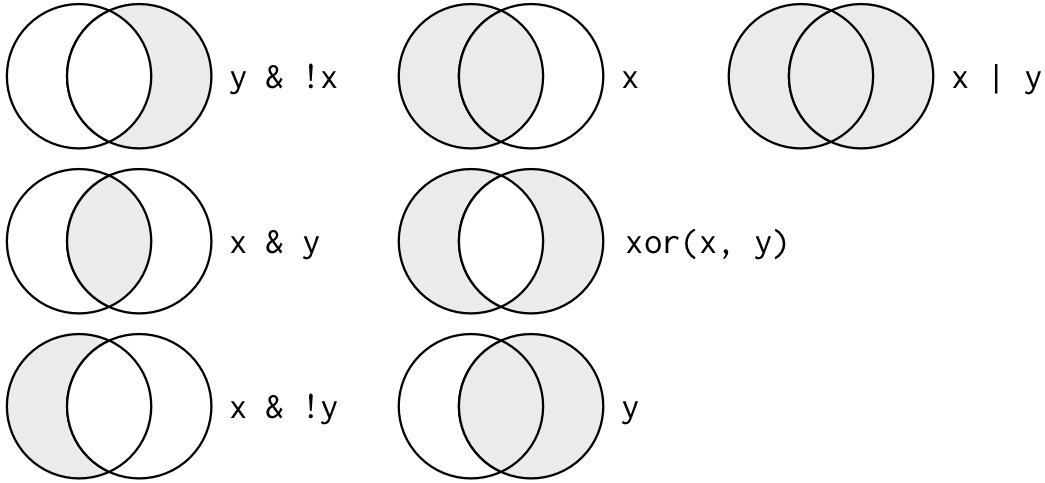
\includegraphics{transform-logical.png}
\caption{Complete set of boolean operations. x is the left-hand circle,
y is the right-hand circle, and the shaded region show which parts each
operator selects.}
\end{figure}

How would you select all flights in May and June?

\hypertarget{missing-values}{%
\subsection{5.2.3 Missing values}\label{missing-values}}

We covered \texttt{NA}s in some of our exercises last week. Hopefully
reading through this section helped reinforce in your mind how
\texttt{NA}s are handled in R and in the \texttt{dplyr::filter}
function.

\hypertarget{exercises}{%
\subsection{5.2.4 Exercises}\label{exercises}}

These are additional practice to those in the book to reinforce the
reading and try by doing. Solutions for each are given below. Our
suggestion is to try first and test your skill.

\begin{enumerate}
\def\labelenumi{\arabic{enumi}.}
\tightlist
\item
  Find all flights that:
\end{enumerate}

1.1 Had an arrival delay of two or more hours (10,034 flights)

1.2 Flew to Houston (IAH or HOU) (9,313 flights)

1.3 Were operated by United, American, or Delta (139,504 flights)

1.4 Departed in summer (July, August, and September) (86,326 flights)

1.5 Arrived more than two hours late, but didn't leave late (3 flights)

1.6 Were delayed by at least an hour, but made up over 30 minutes in
flight (1,819 flights)

1.7 Departed between midnight and 6am (inclusive) (9,373 flights)

\begin{enumerate}
\def\labelenumi{\arabic{enumi}.}
\setcounter{enumi}{1}
\item
  Another useful dplyr filtering helper is between(). What does it do?
  Can you use it to simplify the code needed to answer the 1.7? (hint:
  look up bwetween in the help menu. You'll see the required syntax,
  where x = vector, and left and right at the boundary values. You will
  also need to add an OR statement to include departure times at exactly
  2400 since the dataframe has departures at both 0 and 2400)
\item
  How many flights have a missing dep\_time? What other variables are
  missing? What might these rows represent?
\end{enumerate}

\#solutions: 1.1 k \textless- filter(flights,(arr\_delay \textgreater{}
120)) 1.2 k \textless- filter(flights,dest ==
``IAH''\textbar dest==``HOU'') 1.3 k \textless-
filter(flights,carrier==``DL''\textbar carrier==``UA''\textbar carrier==``AA'')
1.4 k \textless- filter(flights,month==7 \textbar{} month==8 \textbar{}
month==9) 1.5 k \textless- filter(flights,arr\_delay \textgreater120 \&
dep\_delay == 0) 1.6 filter(flights,dep\_delay \textgreater60 \&
arr\_delay \textless(dep\_delay-30))) 1.7 k \textless-
filter(flights,dep\_time==2400 \textbar{} (dep\_time\textless0601)) 2. m
\textless-
filter(flights,between(dep\_time,0,0600)\textbar dep\_time==2400) 3. y
\textless- filter(flights, is.na(dep\_time))

\hypertarget{arrange}{%
\subsection{5.3 Arrange}\label{arrange}}

\begin{enumerate}
\def\labelenumi{\arabic{enumi}.}
\item
  Use desc() to re-order by a column in descending order:
\item
  Sort flights to find the most delayed flights. Find the flights that
  left earliest.
\item
  Sort flights to find the fastest (highest speed) flights. Here you are
  creating a metric by using the existing data in the dataframe to
  calculate speed.
\item
  Which flights traveled the farthest? Which traveled the shortest?
\end{enumerate}

(flights 1632 and 51)

\begin{Shaded}
\begin{Highlighting}[]
\NormalTok{b }\OtherTok{\textless{}{-}} \FunctionTok{arrange}\NormalTok{(flights, distance)}
\end{Highlighting}
\end{Shaded}

\hypertarget{select-columns}{%
\subsection{5.4 Select Columns}\label{select-columns}}

It's not uncommon to get datasets with hundreds or even thousands of
variables. In this case, the first challenge is often narrowing in on
the variables you're actually interested in. \texttt{select()} allows
you to rapidly zoom in on a useful subset using operations based on the
names of the variables.

\texttt{select()} is not terribly useful with the flights data because
we only have 19 variables, but you can still get the general idea:

\begin{Shaded}
\begin{Highlighting}[]
\FunctionTok{select}\NormalTok{(flights, year, month, day)}
\end{Highlighting}
\end{Shaded}

\begin{verbatim}
## # A tibble: 336,776 x 3
##     year month   day
##    <int> <int> <int>
##  1  2013     1     1
##  2  2013     1     1
##  3  2013     1     1
##  4  2013     1     1
##  5  2013     1     1
##  6  2013     1     1
##  7  2013     1     1
##  8  2013     1     1
##  9  2013     1     1
## 10  2013     1     1
## # ... with 336,766 more rows
\end{verbatim}

** Don't worry about 5.4.1 exercises

\hypertarget{add-new-variables}{%
\subsection{5.5 Add new variables}\label{add-new-variables}}

The functions \texttt{mutate} and \texttt{transmute} are used to add new
variables/columns to a data frame.

Following
\href{https://r4ds.had.co.nz/transform.html\#add-new-variables-with-mutate}{the
example at the beginning of section 5.5 in the book}, add a new speed
variable using mutate to your data frame.

\begin{Shaded}
\begin{Highlighting}[]
\NormalTok{flights\_sml }\OtherTok{\textless{}{-}} \FunctionTok{select}\NormalTok{(flights, }
\NormalTok{  year}\SpecialCharTok{:}\NormalTok{day, }
  \FunctionTok{ends\_with}\NormalTok{(}\StringTok{"delay"}\NormalTok{), }
\NormalTok{  distance, }
\NormalTok{  air\_time}
\NormalTok{)}

\CommentTok{\#add a speed variable}
\end{Highlighting}
\end{Shaded}

Now, create a new vector with just the speed vector using transmute.
This allows you to create a new data frame and keep just the new
variables that are calculated.

Next, pay attention to the
\href{https://r4ds.had.co.nz/transform.html\#mutate-funs}{Useful
creation functions} modular arithmetic section to obtain hour and
minutes from the departure data. Try for yourself below. This is pretty
cool and can be useful.

\hypertarget{grouped-summaries}{%
\subsection{5.6 Grouped summaries}\label{grouped-summaries}}

Grouped summaries are essentially what pivot tables are in Excel, if you
have ever heard of those. By using the \texttt{summarise()} function
with the \texttt{group\_by} function we can, for example find the
average flight delay by month. This becomes really awesome! This example
starts with using \texttt{group\_by} to group the data, then applies
\texttt{summarise}.

\begin{Shaded}
\begin{Highlighting}[]
\NormalTok{by\_month }\OtherTok{\textless{}{-}} \FunctionTok{group\_by}\NormalTok{(flights, month)}
\NormalTok{f }\OtherTok{\textless{}{-}} \FunctionTok{summarise}\NormalTok{(by\_month, }\AttributeTok{delay =} \FunctionTok{mean}\NormalTok{(dep\_delay, }\AttributeTok{na.rm =} \ConstantTok{TRUE}\NormalTok{))}
\end{Highlighting}
\end{Shaded}

\hypertarget{last-concept-piping}{%
\subsection{5.6.1 Last concept:: Piping}\label{last-concept-piping}}

In the example above, we ended up with 2 lines of code and created an
intermediate dataframe called by\_month. The second line of code then
used this in the summarise function.

The idea of piping is that it can make it easier to write, follow, and
understand what the commands are doing. Think of each pipe command as
``then''. The pipe command uses the following syntax :
\texttt{\%\textgreater{}\%}. What it essentially does is take the result
of the code on the left-hand side or previous line(s) and pass it as the
first argument to the function on the right-hand side.

We can recreate the example above with pipes. Written in words the code
chunk below would be: ASSIGN a new object name,\\
CHOOSE the dataset to operate on, THEN GROUP the dataset flights by
month, THEN SUMMARIZE the mean of the departure delay.

\begin{Shaded}
\begin{Highlighting}[]
\NormalTok{summary\_FlightDelay }\OtherTok{\textless{}{-}} \CommentTok{\# I like to use a new line here so that I can easily comment out the assignment while building my pipe}
\NormalTok{  flights }\SpecialCharTok{\%\textgreater{}\%}
  \FunctionTok{group\_by}\NormalTok{(month) }\SpecialCharTok{\%\textgreater{}\%}
  \FunctionTok{summarise}\NormalTok{(}\AttributeTok{delay =} \FunctionTok{mean}\NormalTok{(dep\_delay, }\AttributeTok{na.rm =} \ConstantTok{TRUE}\NormalTok{))}
\end{Highlighting}
\end{Shaded}

We'll get to making those sweet, sweet plots soon.

\end{document}
